\chapter{你的头脑是二值逻辑,还是三值逻辑?}\label{chap:w1}

\noindent \href{https://github.com/taseikyo/arts}{readme} | \hyperref[chap:w2]{next}

\begin{figure}[htbp]
  \centering
    
\includegraphics[width=\textwidth]{../images/2020/11/clay-banks-BY-R0UNRE7w-unsplash.jpg}
  \caption{\textit{Photo by Clay Banks on Unsplash}}
\end{figure}

\textit{总字数:1753 个(汉字:1087,英文单词:178,数字:62,中文标点:124,英文标点:302),阅读时长约:3 分 30 秒。}

\section{algorithm \hyperref[chap:w1]{top}}\label{w1:algorithm}

\subsection{\href{https://leetcode-cn.com/problems/sort-integers-by-the-number-of-1-bits}{1356. 根据数字二进制下 1 的数目排序}}

20/11/6 的每日一题,将数组中的元素按照其二进制表示中数字 1 的数目升序排序。思路很简单,直接将数组按照 1 的个数分组,然后排序即可。

\begin{itemize}
  \item \href{https://github.com/taseikyo/arts/blob/master/code/leetcode_1356.cpp}{code/leetcode\_1356.cpp}
\end{itemize}

\begin{lstlisting}[language=C++]
class Solution {
  public:
	vector<int> sortByBits(vector<int>& arr) {
		vector<int> ret;
		map<int, vector<int>> mp;
		for (auto& num : arr) {
			int cnt = 0;
			int tmp = num;
			while (tmp != 0) {
				if (tmp & 1)
					cnt++;
				tmp >>= 1;
			}
			mp[cnt].push_back(num);
		}
		for (auto& iter : mp) {
			sort(iter.second.begin(), iter.second.end());
			for (auto& it : iter.second)
				ret.push_back(it);
		}
		return ret;
	}
};
\end{lstlisting}

\section{review \hyperref[chap:w1]{top}}\label{w1:review}

\subsection{\href{https://nedbatchelder.com/blog/201206/eval_really_is_dangerous.html}{Python 的 eval() 函数很危险(英文)}}

Python 中的 eval() 函数用来执行一个字符串表达式,并返回表达式的值。它的语法如下:

\begin{lstlisting}[language=Python]
eval(expression[, globals[, locals]])
\end{lstlisting}

\begin{itemize}
	\item expression -- 表达式。
	\item globals -- 变量作用域,全局命名空间,如果被提供,则必须是一个字典对象。
	\item locals -- 变量作用域,局部命名空间,如果被提供,可以是任何映射对象。
\end{itemize}

它并不会进行检查,所以即使你传入一个 \lstinline{os.system('rm -rf /')} 这类命令它也会执行,所以这个函数是很危险的。

文中介绍了使用 eval 的 "攻防",先是给出一段代码无法运行,似乎是保证了 eval 函数的安全,但是紧接着立马给出破解的方法,使得 eval 能跑出结果,挺有趣的。

本来是边看边跑文中给出的代码,然而文中的下面这段代码现在无法运行,文中介绍说需要提供 12 个参数,但是放到 ipython 中运行提示说参数不够,需要 14 个,不太懂这段代码的展开,以后有机会再看吧。

\begin{lstlisting}[language=Python]
s = """
(lambda fc=(
    lambda n: [
        c for c in
            ().__class__.__bases__[0].__subclasses__()
            if c.__name__ == n
        ][0]
    ):
    fc("function")(
        fc("code")(
            0,0,0,0,"KABOOM",(),(),(),"","",0,""
        ),{}
    )()
)()
"""
eval(s, {'__builtins__':{}})
\end{lstlisting}

能够直接解析字符串运行的函数似乎都挺危险的,之前了解到 js 中也有这样的问题。算是个双刃剑吧,看使用者如何使用,用在恰当的地方就是好的 feature,被利用来干坏事就是 bug 了。

\section{tip \hyperref[chap:w1]{top}}\label{w1:tip}

\subsection{\href{https://blog.alispit.tel/create-a-git-diff-in-markdown}{如何在 Markdown 文档显示 diff 效果(英文)}}

挺有趣的一个小技巧,之前也有想过怎么显示 diff 效果,后面就忘记去研究了。

\begin{figure}[htbp]
	\centering
	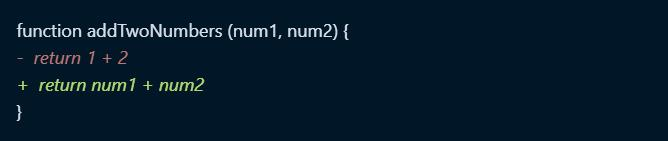
\includegraphics[width=0.8\textwidth]{../images/2020/11/20201106114217}
	\caption{20201106114217.jpg}
\end{figure}

其实也简单,本身就是 md 支持的,用 `diff` 标记语言类型,然后用 `+/-` 表示修改的代码行即可:

\begin{lstlisting}[language=Bash]
function addTwoNumbers (num1, num2) {
-  return 1 + 2
+  return num1 + num2
}
\end{lstlisting}

\subsection{\href{https://dyno-might.github.io/2020/10/30/temperature-conversion-for-the-lazy-and-simple-minded}{华氏度与摄氏度的简单估算(英文)}}

华氏度与摄氏度的转换,有一个简单的估算方法。有三个华氏度,颠倒个位数和十位数,等于对应的摄氏度。

\begin{figure}[htbp]
\centering
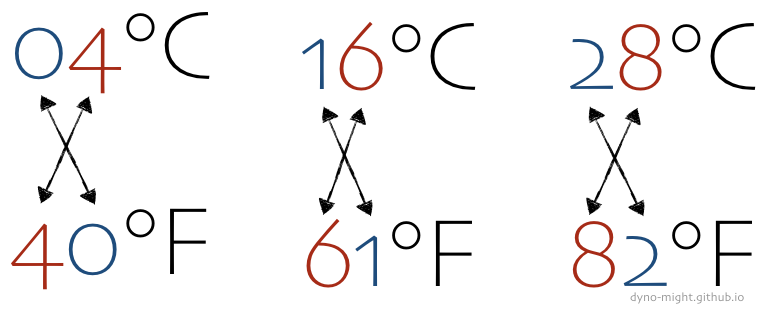
\includegraphics[width=\textwidth]{../images/2020/11/transpose}
\caption{transpose.png}
\end{figure}

因此,记住这三个数字(40、61、82),就可以简单估算:

\begin{table}[h]
    \centering
    \begin{tabular}{|l|l|l|}
    \hline
        摄氏度范围 & 华氏度范围 & 描述 \\ \hline
        < 4\textdegree C & < 40\textdegree F & Cold \\ \hline
        4\textdegree C \textasciitilde 16\textdegree C & 40\textdegree F \textasciitilde 61\textdegree F & Cool \\ \hline
        16\textdegree C \textasciitilde 28\textdegree C & 61\textdegree F \textasciitilde 82\textdegree F & Warm \\ \hline
        > 28\textdegree C & > 82\textdegree F & Hot \\ \hline
    \end{tabular}
\end{table}

\section{share \hyperref[chap:w1]{top}}\label{w1:share}

\subsection{你的头脑是二值逻辑,还是三值逻辑?}

这个话题来自阮一峰的 \href{https://github.com/ruanyf/weekly/blob/master/docs/issue-131.md#%E6%9C%AC%E5%91%A8%E8%AF%9D%E9%A2%98%E4%BD%A0%E7%9A%84%E5%A4%B4%E8%84%91%E6%98%AF%E4%BA%8C%E5%80%BC%E9%80%BB%E8%BE%91%E8%BF%98%E6%98%AF%E4%B8%89%E5%80%BC%E9%80%BB%E8%BE%91}{第 131 期} 科技爱好者周刊,他文中写道:

\begin{myquote}
\textcolor{gray}{我现在的看法是,这可以区分一个人的世界观是否成熟深刻。有些年轻朋友就是二值逻辑的头脑,一看到不赞成、不理解、不喜欢的言论,就认定对方是错误的,完全否定,这其实是思想不成熟的表现。世界太复杂,很难用两分法来判断,三值逻辑会让你的心态好很多,而且有利于个人的进步:正确和错误之间,存在一个广阔的中间地带,任何一种言论都可能有正确的成分,要学会从中间地带去看待事物,吸收对自己有用的部分,摒弃无用的部分。}
\end{myquote}

我比较赞成阮一峰老师的观点,为人处事不是做数学题,在你做完某道数学题后,结果就已经确定了,要么对要么错,但人不是,对于一个陌生人,你能用一个简单标准划分他是好人还是坏人吗?在对与错中间应该还有一个区域,就拿我们学过的牛顿力学一样,在某种条件下它是对的,在另外一种条件下,它又变成错的了。我们得发散地去看待事物,不要非黑即白,应该看到它中间的灰色地带。

两值世界观的人是没长大的小屁孩吧(指特定人群),轻易就能被人煽动,因为他们的思维是非黑即白的,一旦接受白变黑或者黑变白的设定,他们会很有认同感,然后就被牵着鼻子走。令人厌恶的网络喷子大概也是这类人吧。

\noindent \href{https://github.com/taseikyo/arts}{readme} | \hyperref[chap:w2]{next}
